\documentclass[11pt, a4paper]{article} % Consider 'amsart' for publishing

% ===== ESSENTIAL PACKAGES =====
\usepackage{amsmath, amssymb, amsthm} % AMS mathematical facilities
\usepackage{mathtools} % For advanced math formatting (e.g., cases)
\usepackage{geometry} % For adjustable margins
\usepackage{graphicx}
\geometry{a4paper, margin=1in} % Set margins to 1 inch

% ===== CUSTOM THEOREM ENVIRONMENTS =====
\newtheorem{theorem}{Theorem}[section]
\newtheorem{lemma}[theorem]{Lemma}
\newtheorem{proposition}[theorem]{Proposition}
\newtheorem{corollary}[theorem]{Corollary}
\newtheorem{definition}[theorem]{Definition}
\newtheorem{example}[theorem]{Example}
\newtheorem{remark}[theorem]{Remark}

% ===== SHORTCUT COMMANDS =====
% Common sets (mathbb)
\newcommand{\R}{\mathbb{R}} % Real numbers
\newcommand{\N}{\mathbb{N}} % Natural numbers
\newcommand{\Z}{\mathbb{Z}} % Integers
\newcommand{\C}{\mathbb{C}} % Complex numbers
\newcommand{\Q}{\mathbb{Q}} % Rational numbers

% Common operators (mathrm)
\newcommand{\diff}{\mathop{}\!\mathrm{d}} % For integrals: dx -> \diff x
\DeclareMathOperator{\arcsec}{arcsec} % Declare operators that aren't predefined

% ===== DOCUMENT BEGIN =====
\title{Feedback Systems}
\author{Oliver Ekeberg}
\date{\today} % You can remove this for a fixed date or leave blank

\begin{document}
\maketitle

\begin{abstract}
    A note on the book Feedback Systems
\end{abstract}

\section{Introduction}
\label{sec:introduction}

Basic feedback loop: Sensing, computing and acting

In genereal, the feedback system will have some inputs, states and outputs. Illustrated by

\begin{enumerate}
    \item Input : $u(t) $
    \item states : $x(t)$
    \item outputs: $y(t)$
\end{enumerate}




\section{Feedback loop and stability}

Before we get to the Nyquist stability criterion, we need to establish the motivation behind exploring stability. Good performance needs high-gain controllers. Yet, the feedback loop will become unstable if the gain is too high. This is where the Nyquist criterion comes in, it allows us to analyze stability. 

Nyquist criterion involves 


\begin{itemize}
    \item open-loop frequency response function
    \item magnitude
    \item phase
\end{itemize}


Two approaches

\begin{enumerate}
    \item Classical approach in the frequency domain : Single input, single output (SISO)
    \item state-space models : multiple inputs, multiple outputs (MIMO)
\end{enumerate}



\subsection{Standard feedback loop}

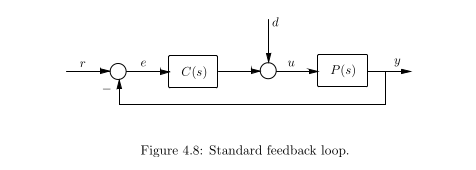
\includegraphics{Standard feedback loop.png}


\subsubsection{closed loop transfer functions}






Nyquist stability criterion determines the stability of a closed loop system based on the Nyquist plot. It states that the stability depends on the number of encirclements of the critical point (-1,0) in the Nyquist plot of the open loop transfer function.


\textbf{\textit{A closed loop system is a system where the outout is compared to a desired refernce output, then the difference becomes an input to the system. An open loop system is a system where the output is not fed back to the input.}}





A closed loop system is stable if the number of encirclements of $ -1 + 0i = N$ in the Nyquist plot is  \[
N = P - Z
\] 

where

\begin{itemize}
    \item \textbf{\textit{P}}: Open loop poles in the right half plane (RHP)
    \item \textbf{\textit{Z}}: Number of closed-loop poles in the RHP
\end{itemize}


\subsection{Applications of Nyquist plot}

\begin{enumerate}
    \item Analysis of closed loop stability
    \item Evaluating \textbf{\textit{stability margins}} and \textbf{\textit{phase margins}}
    \item Designing PID controllers and compensators in control systems
\end{enumerate}



% ===== BIBLIOGRAPHY =====
% Uncomment the lines below if you have references
% \bibliographystyle{plain}
% \bibliography{references}

\end{document}
